En este capítulo contaremos el diseño del proceso de recolección, selección y anotación de datos. Por lo marcado en anteriores secciones, consideramos interesante el problema de hacer una detección de lenguaje discriminatorio bajo un contexto. Es decir, no es lo mismo considerar el mensaje ``sos un hombre'' en solitario que si ese mismo mensaje está dirigido hacia una mujer trans.

Nos abocamos a la decisión de crear un dataset que no sólo contenga un mensaje/comentario, sino que provea un contexto en el cual se da este mensaje. Un ámbito natural para esta tarea son las notas periodísticas, donde disponemos de una nota y comentarios realizados sobre esta. Un ejemplo puede verse . 

Muchos sitios de noticias disponen de sistemas embebidos de comentarios, pero vista la dificultad para la recolección a la vez que los limitados datos provistos por estos sitios nos llevaron a buscar otro medio: Twitter. Twitter provee una sencilla API para descargar datos, a la vez

Algo a tener en cuenta es que este tipo de datos tiene una naturaleza particular, ya que las agresiones discriminatorias son usualmente a personajes públicos o colectivos de personas, y se dan de manera indirecta (a través del comentario en la noticia) y no directa (es decir, como respuesta al usuario de Twitter ofendido)



\section{Recolección de noticias y comentarios}

\begin{table*}[t]
    \centering
    \begin{tabular}{ c|c|c }
        coronavirus  &  encierro          & síntomas \\
        covid        &  fase              & dengue   \\
        cuarentena   &  infectados        & aedes    \\
        normalidad   &  Wuhan             & mosquito \\
        aislamiento  &  distanciamiento   & cacharro \\
        padecimiento &  fiebre            &          \\
    \end{tabular}
    \caption{Words used to retrieve COVID-19 and Dengue related articles.\label{tab:article_words}}
\end{table*}



Usamos la API de Twitter Stream mencionando cualquiera de estas cuentas. Para cualquier tweet de uno de estos medios, reconstruimos la conversación. Para el propósito de este trabajo, solo estamos interesados en el primer nivel de respuestas al tweet original \footnote{Usamos una versión antigua de la API. La versión 2.0 parece facilitar la recopilación de conversaciones}. También eliminamos las URLs de los artículos de los enlaces.


Si bien consideramos otros medios (en particular, los ``periódicos'' electrónicos de derecha) decidimos apostar por medios más tradicionales con apoyo escrito: Clarín (@clarincom), La Nación (@LANACION), Infobae (@infobae), Perfil. (@perfilcom), Crónica (@cronicacom). Como el proceso de anotación iba a ser realizado por anotadores locales, decidimos no recopilar ningún dato de otros países de habla hispana.


El foco se hizo en artículos relacionados con COVID-19. Para ello, seleccionamos artículos buscando una cantidad de palabras en su cuerpo, por lo que seleccionamos específicamente artículos relacionados con COVID-19. La tabla \ref{tab: article_words} contiene las palabras utilizadas para recuperar estos artículos. También estábamos interesados en la pandemia del dengue; sin embargo, solo se recuperó un número muy pequeño de artículos.


\subsection{Diarios elegidos}

Para esta tarea, elegimos 5 diarios:

\begin{itemize}
    \item Clarín
    \item La Nación
    \item Infobae
    \item Perfil
    \item Crónica
\end{itemize}

Estos diarios son los mayores generadores de contenido. Consideramos otros medios, pero nos atuvimos a medios formales tradicionales y con soporte escrito. 

En un principio consideramos la posibilidad de anotar tweets de digiarios de otros países, pero teniendo en cuenta que esta tarea depende fuertemente de la jerga y de las variaciones dialectales de cada país decidimos realizar sólo anotación de estos diarios. A su vez, observamos que la mayoría de los comentarios son de la variedad dialectal rioplatense 


\subsection{Datos recolectados}

\begin{table}[t]
    \centering
    \begin{tabular}{c|c|c}
    Medio      & \#Artículos recolectados & \#Comentarios \\
    \hline
    @infobae   &  45652   &  822462 \\
    @clarincom &  29050   &  672401 \\
    @perfilcom &  8764    &  61203  \\
    @LANACION  &  16040   &  506091 \\
    @cronica   &  17250   &  70872 \\
    \hline 
    Total      & 116756  & 2133029 \\
    \end{tabular}
    \caption{Artículos recoletados por medio}
    \label{tab:articulos_recoletados_por_medio}
\end{table}


En la tabla \ref{tab:articulos_recoletados_por_medio} damos los números de los artículos recolectados por cada medio, luego de aplicado . Si bien recolectamos más artículos de otros medios, no son enumerados. Infobae es el medio que más producción de artículos genera, y también será finalmente sobre el que más comentarios etiquetemos.

La figura \ref{fig:fecha_articulos_por_medio_todas} muestra la distribución temporal de los artículos, sin aplicar ningún filtro por palabras, mientras que \ref{fig:fecha_articulos_por_medio_covid} muestra aquellas relacionadas al COVID-19 utilizando el filtro de palabras listado en la tabla \ref{tab:article_words}. Podemos observar dos caídas. Hay un pequeño pozo en mayo 2020 que se debió a la caída de nuestros servidores de recolección. Por otro lado, observamos que algunos medios (particularmente La Nación) parecieran mencionar menos directamente al COVID (al menos con los términos referidos anteriormente) hasta un nuevo pico cerca de fin de año, coincidente con un nuevo rebrote del virus en este país. 

Sin embargo, todo esto puede ser un artefacto del método de filtrado: muchas notas contienen links a otras con sus títulos y eso puede interferir en estas estimaciones. Así y todo, decidimos mantener este método ya que consideramos que mayormente las notas en el período referido tienen relación con la pandemia.

\begin{figure}
    \centering
    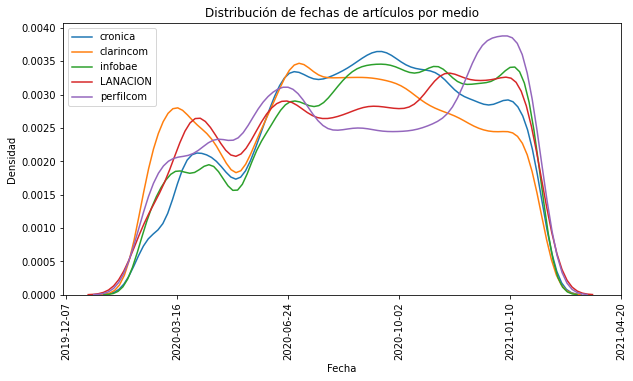
\includegraphics[width=\textwidth]{img/fechas_por_medios_todas.png}
    \caption{Distribución temporal de artículos recolectados}
    \label{fig:fecha_articulos_por_medio_todas}
\end{figure}



\begin{figure}
    \centering
    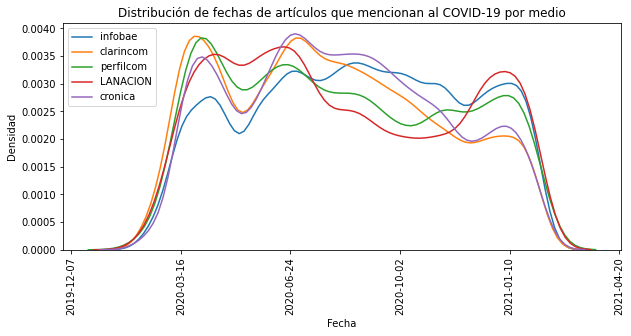
\includegraphics[width=\textwidth]{img/fechas_por_medios.png}
    \caption{Distribución temporal de artículos recolectados que mencionan COVID-19 o algún término relacionado}
    \label{fig:fecha_articulos_por_medio_covid}
\end{figure}



\section{Selección de datos a anotar}


Un problema que se nos presenta antes de comenzar el etiquetado es el de seleccionar los artículos que vamos a etiquetar. Una primera posibilidad para hacer esto es realizar una selección aleatoria de artículos y comentarios; sin embargo, los comentarios discriminatorios no se distribuyen de manera uniforme entre los artículos, sino que se concentra en algunos temas. Es mucho más probable encontrar comentarios de índole discriminatoria en notas que tengan temas cercanos a alguna de las características protegidas; por ejemplo, es esperable que encontremos contenido odioso en notas sobre China y el Coronavirus o sobre una chica transgénero antes que en un artículo de fútbol o economía. 


Teniendo esto en cuenta, evaluamos varias alternativas. La primera es observar los artículos e intentar seleccionar aquellos que consideremos que puedan tener contenido potencialmente discriminatorio. 

Una posibilidad para esto sería usar algunas palabras ``semilla'' para seleccionar artículos interesantes. Otra sería buscar directamente comentarios que contengan algunos insultos comunes o expresiones peyorativas hacia nuestros grupos protegidos. Después de algunos experimentos, decidimos utilizar el muestreo basado en comentarios.

\subsection{Selección en base a artículos}

En primer lugar, consideramos la posibilidad de hacer una selección en base al contenido de los artículos. Luego de realizar algunos experimentos usando LDA \cite{blei2003latent} para buscar tópicos posibles de las notas, decidimos realizar una selección un poco más controlada y determinística en base a la utilización de palabras clave. Es decir, seleccionaremos artículos en base a la aparición o no de ciertas ``semillas''

Para ello, indexamos todos nuestros artículos en MongoDB \footnote{\url{https://www.mongodb.com/}}, una base de datos no relacional y desestructurada. MongoDB permite la utilización de índices en base a texto, y realizar búsquedas en base a textos, palabras, e inflexiones. Cada artículo fue indexado en base al contenido de su cuerpo (es decir, el texto en sí del artículo).

La tabla \ref{tab:palabras_articulos} muestra el conjunto utilizado para recolectar artículos. Como vemos, hay diversas palabras que recogen distintas temáticas de posibles tópicos ``calientes'', algunos muy locales respecto a eventos concretos durante la pandemia. 

\begin{table}[]
    \centering
    \begin{tabular}{l | l | l | l}
    China        &  piqueteros              &  mamá                & empleadas domésticas  \\ 
    Cuba         &  villas                  &  de género           & la modelo             \\               
    cubano       &  la villa                &  aborto              & la periodista         \\            
    bolivia      &  movimientos sociales    &  actriz              & la cantante           \\               
    paraguayo    &  organizaciones sociales &  actrices            & travesti              \\               
    judío        &  tomas de tierras        &  feminista           & trans                 \\                 
    camionero    &  toma de tierras         &  femicidio           & gay                   \\               
    ladrón       &  sindicatos              &  enfermera           & homosexual            \\                 
    represión    &  Guernica                &  madre               & de la V               \\           
    criminal     &  mapuches                &  personal doméstico  & Ofelia                \\                      
    \end{tabular}
    \caption{Palabras utilizad}
    \label{tab:palabras_articulos}
\end{table}

\subsection{Selección en base a comentarios}

Otra posibilidad es mirar los comentarios de los artículos en lugar del contenido del artículo, y seleccionar posibles temas en base a esto. En este punto, la idea es únicamente seleccionar los artículos y no los comentarios; estos últimos son sólo usados como indicios para ver comentarios con posible contenido discriminatorio, y como tal identificar a ese artículo como un posible generador de este tipo de contenido. 

La idea es similar a la de la selección con artículos, sólo que aplicada a comentarios: buscamos comentarios que contengan alguna de las palabras semilla listadas en la Tabla \ref{tab:palabras_comentarios}. Estas palabras fueron recolectadas a base de experimentación y observación de los datos, y tratan de contener 

Una idea también considerada fue la de utilizar un clasificador entrenado sobre otro dataset (por ejemplo, el de \citet{hateval2019semeval}) y con eso marcar comentarios posiblemente discriminatorios. Sin embargo, muy probablemente detectaríamos sólo comentarios para las categorías/características etiquetadas en esos datasets e ignorarían las que agregamos en nuestro trabajo; por ejemplo, la mayoría de los datasets no contienen comentarios anotados contra la comunidad LGBTI.

El procedimiento de selección consta de, dado un artículo, marcar sus comentarios que contengan una o más de las expresiones listadas. Si el artículo tiene tres o más comentarios marcados, entonces seleccionamos el artículo; caso contrario, es descartado. 

Vale remarcar que este proceso de selección es para los \emph{artículos}, no para los comentarios.




\begin{table*}[t!]
    \centering
    \begin{tabular}{l|l|l|l|l|l|l}
    bija          & urraca     & viejo puto    & trolo      & peruano  & matarlos         & negra      \\
    prostituta    & tucán      & trabuco       & sodomita   & peruca   & una bomba        & negro de   \\
    feministas    & putita     & travesti      & chinos de  & judío    & vayan a laburar  & negros     \\
    feminazis     & reventada  & trava         & bolita     & sionista & vayan a trabajar & bala       \\
    aborteras     & marica     & degenerado    & paraguayo  & villeros & gorda            & uno menos  \\
    \end{tabular}
    \caption{Palabras utilizadas para recolectar comentarios}
    \label{tab:palabras_comentarios}
\end{table*}



Luego de algunos análisis experimentales y observacionales de las dos posibles metodologías, decidimos utilizar el muestreo de artículos en base a comentarios. Por lo que pudimos observar, los artículos seleccionados parecían tener mayor incidencia de mensajes odiosos y eso nos decantó hacia esa opción. 

\section{Criterios de anotación}
\label{sec:criterios}

La definición de lenguaje discriminatorio utilizada en este trabajo está basada en trabajos de la Comisión Interamericana de Derechos Humanos (CIDH)\cite{CIDH2015}, del Centro de Estudios de Libertad de Expresión (CELE) \cite{cele2019} y en el Article 19 Hate Speech Toolkit \cite{article192015}. 

Teniendo estos insumos en cuenta, entendemos que hay discurso discriminatorio en un texto social si contiene declaraciones de carácter intenso y posiblemente irracional de rechazo, enemistad y aborrecimiento contra un individuo o contra un grupo, siendo estos objetivos de estas expresiones por poseer (o aparentar poseer) una característica protegida.

Las características en cuestión son protegidas por leyes internacionales. En este trabajo consideramos las siguientes:

\begin{enumerate}
\item Sexo (Mujeres, concretamente)
\item Género o identidad sexual (Colectivo LGBTI)
\item Ser inmigrantes, extranjeros, pueblos aborígenes u otras nacionalidades (xenofobia, racismo)
\item Situación socioeconómica o barrio de residencia
\item Poseer discapacidades, problemas salud mental o de adicción al alcohol, drogas u otros estupefacientes
\item Opinión o ideología política
\item Aspecto o edad (mayormente, gordofobia/gerontofobia)
\item Antecedentes penales o estar privado de la libertad
\end{enumerate}

Si bien algunas de estas características no son consideradas en algunos tratados (por ejemplo, contra los presos), las tuvimos en cuenta por las características propias del tratamiento en medios durante la pandemia de distintos sucesos.


\section{Modelo de etiquetado}

Un modelo de anotación es, según \citet{pustejovsky2012natural}, una representación práctica del objetivo de anotación. En nuestro caso, queremos marcar comentarios discriminatorios, marcar a qué grupos y/o características se está ofendiendo, y también identificar llamados a tomar alguna acción contra los objetos de esos discursos. Por lo pronto, haremos una definición que capture ese objetivo sin deternos demasiado en especificarlo formalmente (lo que llaman en ese libro ``especificación''). 

\subsection{Modelo Jerárquico de Etiquetado}
\citet{zampieri2019predicting} introdujeron un modelo jerárquico de anotación para la tarea de lenguaje ofensivo, utilizado en las competiciones OffensEval \cite{zampieri2019semeval2019} y hatEval \cite{hateval2019semeval}. La idea de la anotación jerárquica es realizar anotaciones adicionales sólo para algunos casos de anotaciones del nivel anterior. 

En el caso de \emph{HatEval}, tenemos un primer nivel que consta de anotar si un tweet contiene o no lenguaje de odio (nivel 1). Si el tweet tiene lenguaje de odio, entonces anotamos si está dirigido a un individuo o a un grupo, y también anotamos si es agresivo o no (ambos nivel 2). En el caso de \emph{OffensEval}, primero anotamos si es ofensivo (nivel 1), luego si está dirigido o es un insulto no dirigido (nivel 2) y finalmente, si es dirigido y ofensivo, marcamos su objetivo (nivel 3). En la figura \ref{fig:modelos_offenseval_hateval} ilustramos ambos modelos. 


%
%
% Link: https://docs.google.com/drawings/d/1ZgTmvRwMWn0B-kokfw87jfSa7eY5-OSBHwltetnNT08/edit
%
 \begin{figure}
     \centering
     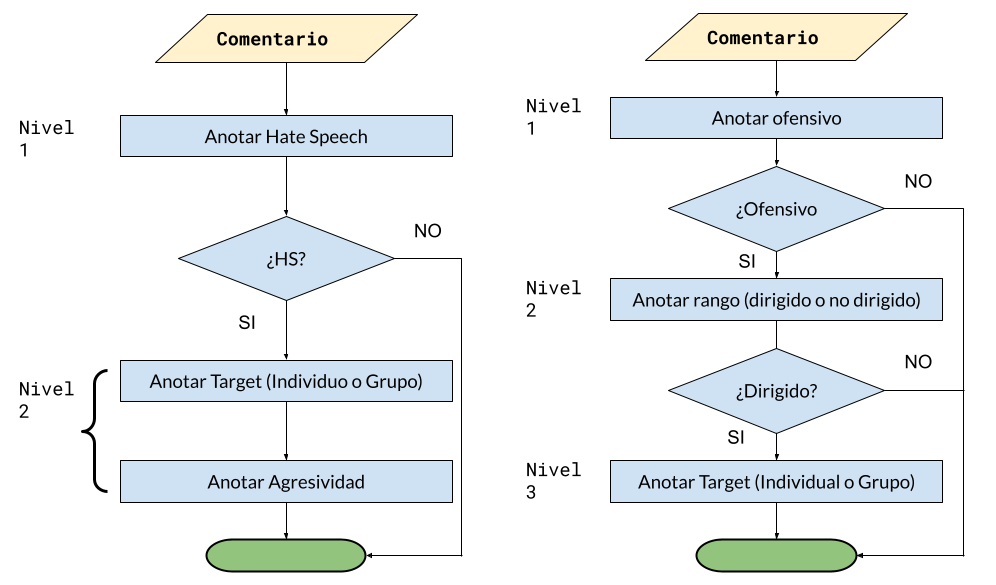
\includegraphics[width=\textwidth]{img/modelosjerarquicos.png}
     \caption{Modelos jerárquicos de anotación. A la izquierda, tenemos el modelo jerárquico propuesto para HatEval \cite{hateval2019semeval}, a la derecha el modelo propuesto para OffensEval \cite{zampieri2019semeval2019}}
     \label{fig:modelos_offenseval_hateval}
 \end{figure}

\subsection{Modelo de etiquetado jerárquico y contextualizado}



\begin{figure}
    \centering
    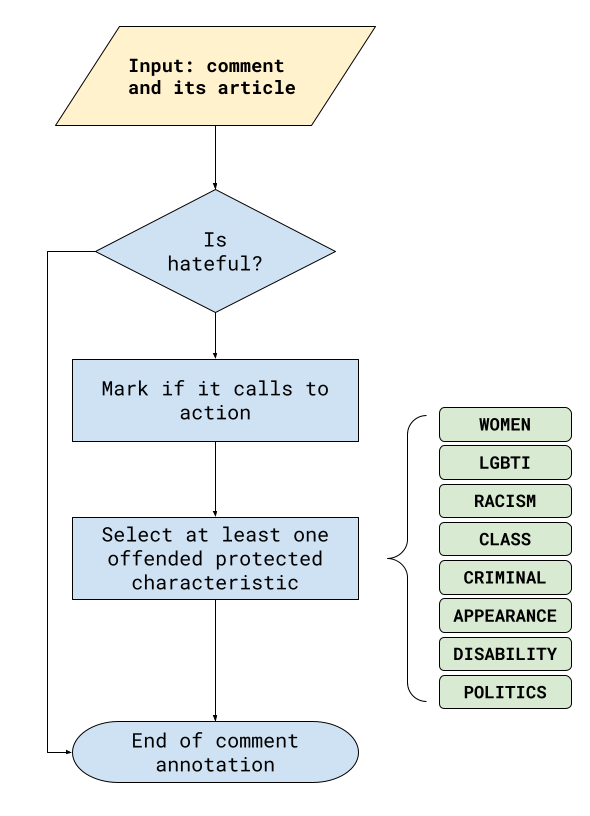
\includegraphics[width=0.70\textwidth]{img/Annotation Model.png}
    \caption{Modelo de anotación}
    \label{fig:annotation_model}
\end{figure}


La figura \ref{fig:annotation_model} muestra el modelo de anotación utilizado. Seguimos un modelo jerárquico similar al propuesto por \citet{zampieri2019predicting}, aunque de sólo un nivel. Para cada comentario y su respectivo contexto (el artículo), requerimos una anotación  para decidir si el comentario es odioso o no. Si no es odioso, no se necesita más información. Si es así, el par artículo-comentario debe contener, además, una anotación por si llama o no a la acción, y al menos una categoría protegida 




\section{Herramienta de etiquetado}

\section{Etiquetadores}

A diferencia de otros trabajos (como hatEval \cite{hateval2019semeval}), decidimos por un lado, garantizar que nuestros anotadores estén más cercanos culturalmente al problema en cuestión, a la vez que tener mayor control del perfil de estos. Consideramos que el discurso de odio tiene un fuerte componente cultural, muchas veces expresado a través de jerga o expresiones dialectales muy particulares, y relacionado con noticias muy propias de esta región.


\subsection{Tipos de anotación en otros trabajos}

Comentar otros trabajos acá

\begin{itemize}
    \item Davidson
    \item Waseem
    \item hatEval
    \item CONAN
    \item Gao (contextualizado)
    \item Context offensive (el de Google, y el griego)
\end{itemize}

\subsection{Perfil de etiquetadores}

Para la selección de anotadores, realizamos una búsqueda interna. Puntualmente, buscamos:

\begin{itemize}
    \item Estudiantes/graduades de carreras de Cs. Sociales, Psicología, Letras o afines
    \item Hablantes nativos (o casi) de Español Rioplatense
    \item Usuarios de redes sociales; preferentemente Twitter
\end{itemize}

Luego de una breve entrevista donde les contamos el proyecto y corroboramos que efectivamente sean hablantes nativos de Español Rioplatense y usuarios de RRSS, les mandamos una pequeña evaluación paga que constó de leer el manual de criterios de anotación (que agregamos en \ref{app:manual_criterios_anotacion}) y anotar 5 artículos. Esto lo realizamos para ver que efectivamente estén entendiendo la tarea. Estos artículos fueron luego reutilizados para el proceso de entrenamiento.

\section{Proceso de etiquetado}

\subsection{Preprocesado de los datos}

\subsection{Entrenamiento de etiquetadores}
\subsection{Esquema de anotación}
Acá anotar los 3 anotados, etc

%
% Esto quizás va después
%

\section{Dataset resultante}
\subsection{Estadísticas}
\subsection{Asignación}
\subsection{Agreements}
\subsection{Recursos utilizados}
\subsection{Anonimización para publicación de los datos}

